\documentclass[11pt,a4paper]{article}
\title{Simulation Assignment Report}
\author{Laurens van den Brink (insert student number) and Nadia Boudewijn 3700607}
\date{\today}

\usepackage{graphicx}
\begin{document}

\begin{titlepage}
\maketitle{}
\end{titlepage}


\tableofcontents
\clearpage



\section{Introduction}
This is report accompanies a simulation model for a production line of DVD's. This simulation model is designed for the Simulation Assignment for the simulation course  2013-2014 at Utrecht University.
\subsection{Problem description}
We will be performing a simulation study for a production line of DVD's, hoping to find improvements for the line. At some points in the line there is limited buffer space and part of the productin is batch processing. The producing company wants to find out the best buffer- and batch sizes to increase the dvd production. They are also interested in possible improvements iof their production line, especially in alleviating the impact of bottlenecks. 

To gain insight on the production line we questioned the domain expert Marjan van den Akker. She provided us with information about the production process. A schematic overview of the production line can be found on the next page. 
\subsection{Project goal}
The goal is to perform a scientific sound simulation study in order to determine if it's possible to increase the DVD production productivity. 
\section{Problem Analysis}
In this section we will discuss the methods we have used to reach the project goal, as well as some domain-specific issues to this simulation study that need to be adressed. 

\begin{figure}
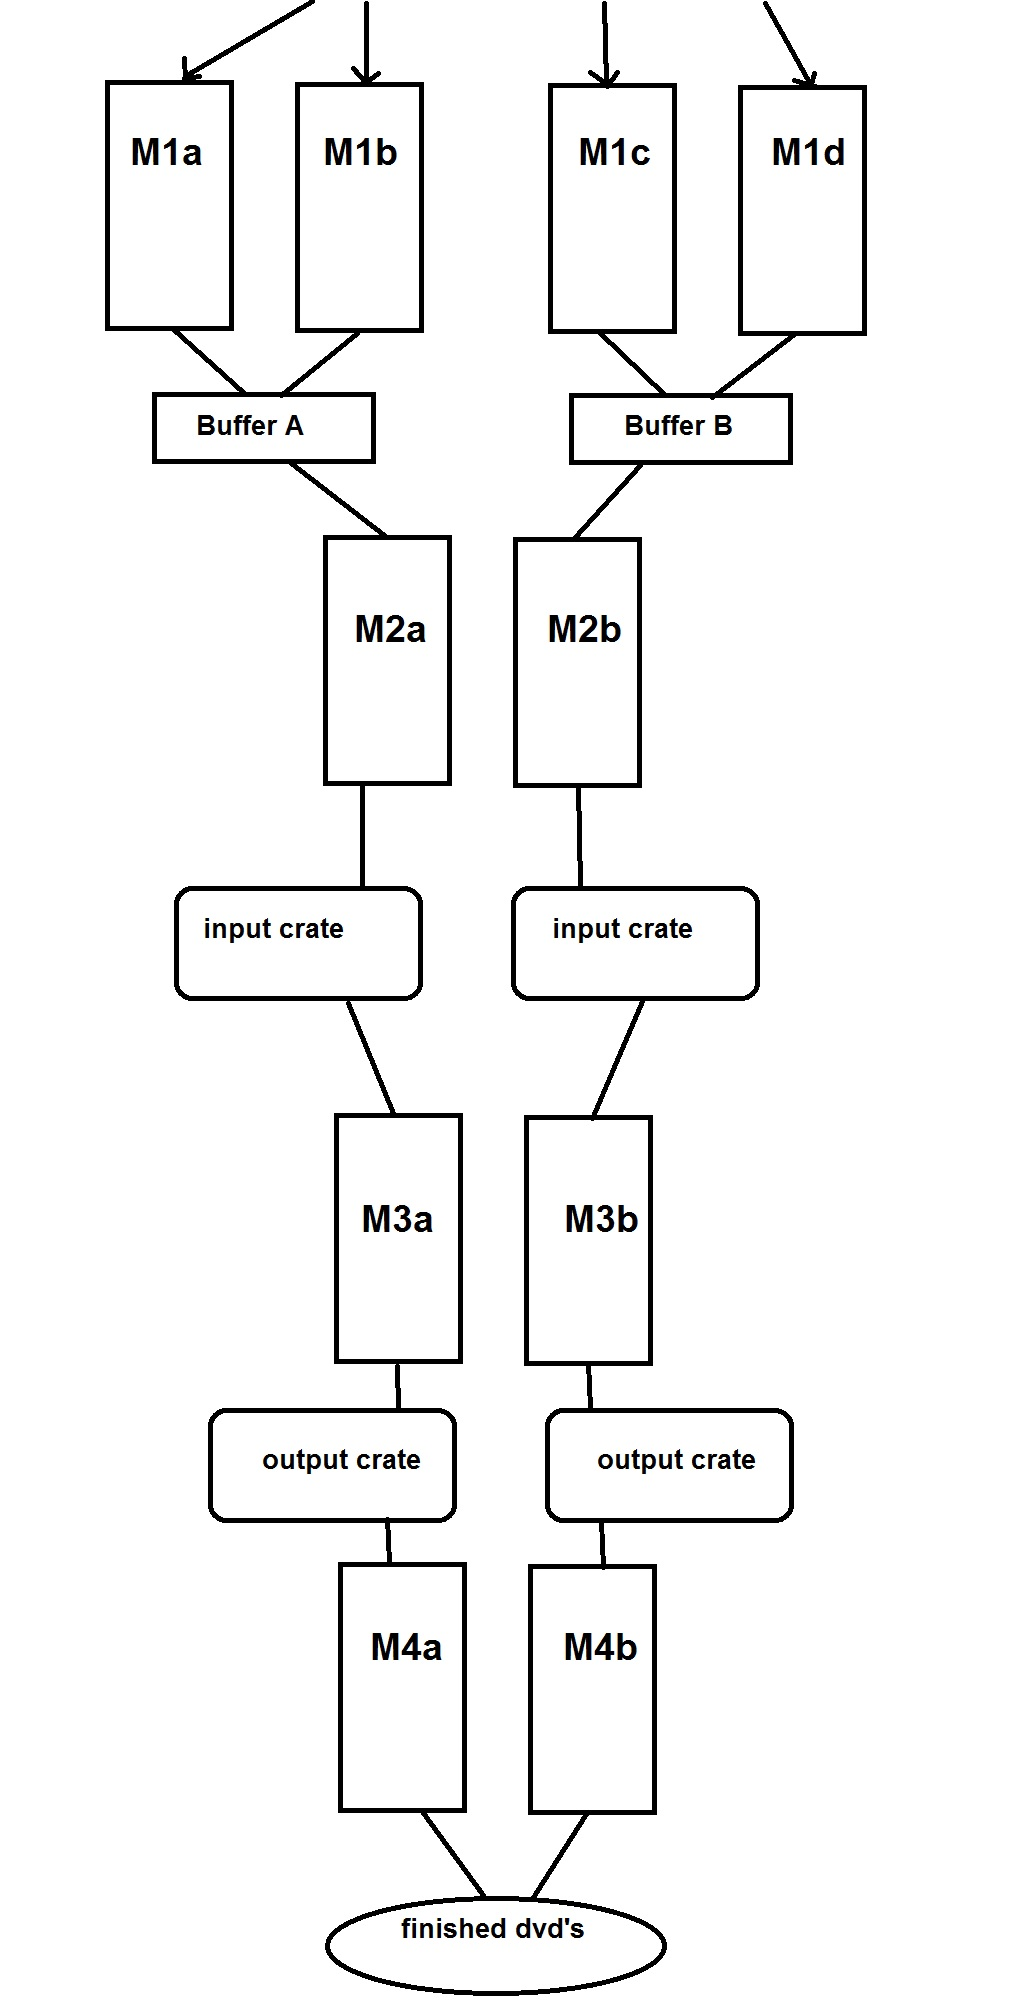
\includegraphics[width = 350 pt]{schemaPL.jpg}
\caption{Schematic representation of the DVD production line}


\end{figure}
\subsection{Assumptions}
A model is supposed to be a simplification of reality, therefore in order to create our model we made some simplifying assumptions that we will discuss in this section. 

\subsubsection{General assumptions}
\begin{itemize}
\item All machines have enough resources available, when they run out, recourses are being refilled immediately (which may cause the machine to stop it's production for some time during the refill).
\item The production line runs 24/7.
\item When we start the production line we assume none of the machines is broken down.
\item At any moment in time enough repairman are available, so that repairs can be scheduled immediately. 
\item Distributions for time to failure and time to repair are equal for machines of the same sort (machines with the same number in our case).
\end{itemize}


\subsection{Model explanation}
We will start with detailed descriptions of each subsystem in bullet format and how these subsystems interact. Next we will give an overview of the events for this model, and how they are handled. We will also discuss the model state and the performance measures, followed by limitations of the simulation model. 

\subsubsection{M1}
Machine 1 - Injecton Molding
\begin{itemize}
\item There are 4 injection machines (M1a, M1b, M1c, M1d)  that may break down individually. 
\item  A machine will break down every 8 hours on average. We implement this with an exponential distribution on the advice of the expert. 
\item  Repairing a machine takes 2 hours on average. We implement this with an exponential distribution on the advice of the expert. 
\item  There is a buffer (B1) for 20 dvd's between M1a, M1b and M2a. Another buffer (B2) that can hold 20 dvd's is placed between M1c, M1d and M2b. 
\end{itemize}

\subsubsection{Buffer}
\begin{itemize}
\item Buffer A and B can each store 20 DVD's
\item Buffer A can be filled by M1a and M1b, and offers DVD's to M2a
\item Buffer B can be filled by M1c and M1d, and offers DVD's to M2b
\end{itemize}

\subsubsection{M2}
Machine 2 - Dye coating and drying
\begin{itemize}
\item  There are 2 machines, M2a and M2b. 
\item A machine ruins 2% of the dvd's. These dvd's get thrown away at the end of the whole production line. 
\item  There is 5 minutes travel (drying time) between M2 and M3. 
\end{itemize}

\subsubsection{Crate}
\begin{itemize}
\item There are 6 crates.
\item Three of these crates can be filled by M2a and  can go into the production of M3a. The other three crates can be filled by M2b and go into production of M3b.
\item These crates are in te most ideal case: an input, an output and a processing crate. But it is possible for the 3 crates to be all input, or all output but only 1 crate at a time can be processed by a M3 machine. 

\end{itemize}
\subsubsection{M3}
Machine 3 - Sputtering, lacquer coating and drying
\begin{itemize}
\item There are 2 machines, M3a and M3b. 
\item  A machine only works on batches of size 20.
\item A batch is stored in a crate
\item  3 percent of de dvd's are in a delayed batch due to cleaning time of the sputtering part. 
\item  On avergage it takes 5 minutes to clean the sputtering part.  We implement this with an exponential distribution on the advice of the expert. 
\item If the sputtering part doens't have to be cleaned the sputtering takes 10 seconds on average per dvd. We implement this with an exponential distribution on the advice of the expert. 
\item Lacquer coating takes 6 seconds on average per dvd. We implement this with an exponentiall distribution on the advice of the expert. 
\item At the end the whole batch needs 3 minutes of drying before it's ready for output. 
\end{itemize}

\subsubsection{M4}
Machine 4 - Printing and Finishing
\begin{itemize}
\item  There are 2 machines, M4a and M4b. 
\item On average, after printing 200 dvd's the inkt will have to be refilled. We implement this with a normal distribution on the advice of the expert. 
\item Replacing the inkt takes 15 minutes on average, with a standard deviation of 1 minute.
\end{itemize}

\subsubsection{Events and event handlers}
TODO: check of de input en output voor elke machine uit eigen buffer is, m1m2
We distinguish te following events:
\begin{itemize}
\item M1Finished
\item M2Finsihed
\item AddDVDToCrate
\item M3Finished
\item M4Finished
\item BreakdownM1
\item RepairedM1
\item BreakdownM3
\item RepairedM3
\item BreakdownM4
\item RepairedM4
\end{itemize}

We use the following eventhandlers to deal with the events: (worden pas ingevoegd als ze compleet zijn)



\subsubsection{Performance measures}
We used the following performance measures:
\begin{itemize}
\item Production per hous: before the simulation study the production was 175 dvd's per hour. We hope to raise this to 200 dvd's per hour. 
\item Throughput time of products 
\end {itemize}


\subsubsection{State}
To keep track of the model state we measure the following:
\begin{itemize}
\item Number of dvd's in production.
\item State of every machine (IDLE / BUSY / BROKEN / WASBROKEN)
\item Buffercontent
\item cratesReadyforInputM3: the amount of crates ready for input M3
\item cratesReadyforInputM4: the number of dvd's that are ready for input M4
\end{itemize}

\subsubsection{Limitations}

\section{Experiments}
Met deze dingen kunnen we rekening houden:
Candidates for sensitivity analysis:
\begin{itemize}
\item the value of a parameter - if it's not sensitive for a specific range of values a better specification is needed
\item  the choice of a distribution
\item  the entity moving thourgh the simulated system - following 1 dvd or a whole batch may produce the same results for the perfomance measures of interest while reducing execution time
\item the level of detail for a subsystem
\item  what data are the most crucial to collect 
\end{itemize}
When one is performing a sensitivity analysis, it is important to use the method of common random numbers to control the randomness in the simulation. Otherwise, the effect of changing one factor may be cofounded with other changes (e.g. different random values from some input distribution) that inadvertently occur.

\subsection{Set up}
Summaries of a data set such as its sample mean and a histogram. Details are for the appendix to retain readability. 
If one has fitted a theoretical probability distribution to a set of observed data, then the adequacy of the representation can be assessed by using the graphical plots and goodness-of-fit tests. 
\subsection{Results}

\subsubsection{Validation}
Establish that the output data closely resembles the output data that would be expected from the actual system. 

Establish the ability to predict future behavior. Use one data set for calibration and another independent set for validation.

\section{Conclusions}

\section{Appendix}

\subsection{Interview notes}

\subsection{Detailed statistical analyses}





\end{document}

